% Chapter 1

\chapter{Chapter 1: Introduction} % Main chapter title

\label{Chapter 1} % For referencing the chapter elsewhere, use \ref{Chapter1} 


%----------------------------------------------------------------------------------------
\section{Introduction to Sequential Decision Making}
\paragraph{}
We are making all kinds of decision in our daily life: whether bringing an umbrella, which canteen shall we go for today's lunch, doing homework or housework, etc. Some daily decisions are sequential, which means that the consequence of an action may reveal its effect in the future, or several sequential actions are required to gain the reward. For example, if you are driving a car on a highway, suddenly you spot a car accident ahead. At this time, you must hit the break and then rotate your steering wheel to avoid another car accident. Only hitting break will result in crashing, though with a lower speed. Only rotating your steering wheel on a high speed situation will make you lose control of the car, most likely making another disaster. Only when you hit the break to slow down the vehicle and then change car's direction can you solve the puzzle. This is a typical sequential decision making problem. Every action you take may cause a consequence, but most importantly, it will influence the consequence of the following actions. 
\paragraph{}
Another representative example is chess. When it is your turn, you can take your time to think about the situation now on the board. After you have made the decision, like moving a rook, you could take your action. This action may have a direct consequence, like eating your opponent's queen. But it also has subsequent consequences, such as your rook being eaten by your opponent's knight. It could also have a far-away consequence, for instance, you lose the game. 
%----------------------------------------------------------------------------------------


%----------------------------------------------------------------------------------------
\section{Introduction to Markov Decision Process}
\paragraph{}
Markov decision process (MDP) provide a mathematical framework for modeling sequential decision making with some restricts. To introduce MDP, we first need to define several terms. At each time step in a MDP, the process is in some state $s$, and the decision maker may choose any action $a$ that is available in state $s$ (\cite{bellman1957markovian}). The process responds at the next time step by randomly moving into a new state $s^{\prime}$, and giving the decision maker a corresponding reward $R(s^{\prime})$. The process is shown in Fig. \ref{fig:MDP}. 

\begin{figure}[ht]
\centering
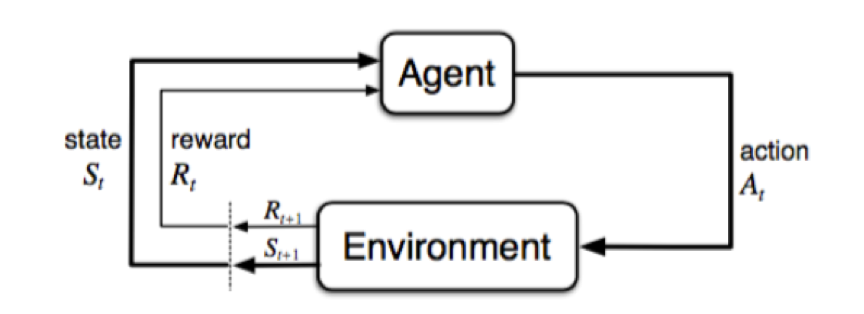
\includegraphics[width=\columnwidth]{Figures/MDP}
\decoRule
\caption[Markov Decision Process]{Markov Decision Process (\cite{sutton1998introduction})}
\label{fig:MDP}
\end{figure}

\paragraph{}
Taken the chess example again, each time the player receive a state $s$, in this case, the chess board situation. The player could choose an action that is viable under current state $s$. Assume the player chooses action $a$, the environment, in this case, the chess rule, will transit the state $s$ into a new state $s^{\prime}$, also giving the player a reward $r$. The reward may be small when you eat a pawn while it may be big when you win the game. 
\paragraph{}
One core property of Markov decision process is that the transition obeys Markov property. Markov property means the probability that the process moves into its new state $s^{\prime}$ is influenced only by the chosen action $a$ and current state $s$. Specifically, it is given by the state transition function $T(s,a,s^{\prime})$. Given $s$ and $a$, it is conditionally independent of all previous states and actions. 
\paragraph{}
Markov property makes it possible to analyze the action selection by only looking at the current state because current state contains all information the decision maker need to know, otherwise the Markov property is unsatisfied. It is obvious that the chess example has Markov property since the information on board, $s$, is sufficient for the player to make its action and transit to a new state (ignore the influence to board caused by opponents). 
% TODO MDP consist of S,A,T,R,\gamma
\paragraph{}
This thesis will focus on Markov decision process only because of the simplicity of Markov property. 
%----------------------------------------------------------------------------------------



%----------------------------------------------------------------------------------------
\section{Thesis Structure}
\paragraph{}
Sequential decision making are so essential that our life may fall apart without such ability. Hence, there has been much work inspecting the process of sequential decision making, especially Markov decision process. In this thesis, I will also try to design an experiment to explore several possible decision methods under Markov devision process. 
\paragraph{}
We have given introduction of the sequential decision making problem and its formalized framework Markov Decision Process in Chapter \ref{Chapter 1}. We will introduce several existing work in this topic in Chapter \ref{Chapter 2}. After that, we will present our experiment in Chapter \ref{Chapter 3}. Chapter \ref{Chapter 4} will be basic statistical analyses and in Chapter \ref{Chapter 5} we will put forward several models that are theoretically possible in our task and compare them with classic ones. Finally, we will discuss and conclude what we have discovered with some future research directions. 
%----------------------------------------------------------------------------------------